\section{Proposed Scheme}\label{sec:method}

\subsection{Problem Formulation}
We model the mainline of Taiwan National Freeway No.~5 as a set of $K=10$ directed ETC gantry segments (5 southbound from 0.0K to 49.4K and 5 northbound from 52.8K to 0.1K), selected from mainline \texttt{05F} gantry pairs with $\ge 90\%$ valid training coverage. Time is discretized into 5-minute slots $t \in \{0, 1, \dots, 287\}$ per day. For segment $k$ at slot $t$, the roadside telemetry provides passenger-car (vehicle class 31) median speed $v_k(t)$ (km/h) and traffic volume $q_k(t)$.

We define a binary congestion indicator using a project-defined threshold $\tau = 40$~km/h:
\begin{equation}
c_k(t) = \mathbb{I}\!\left[v_k(t) < 40\right].
\label{eq:cong_ind}
\end{equation}
Given a query at decision time $T$ (slot $t$) for segment $k$ with historical observations up to $t$ and calendar metadata known prior to $T$, the prediction engine estimates multi-horizon future speed $\hat{v}_k(t+h)$ and calibrated congestion probability $\hat{p}_k(t+h)$ for horizons $h \in \{3, 6, 12\}$ slots ($+15, +30, +60$~minutes):
\begin{equation}
\hat{v}_k(t+h) = f_{\text{reg}}^{(h)}(\mathbf{x}_{k,t}), \qquad
\hat{p}_k(t+h) = g_{\text{cal}}^{(h, s_{k,t})}\!\left(f_{\text{clf}}^{(h)}(\mathbf{x}_{k,t})\right),
\label{eq:forecast}
\end{equation}
where $\mathbf{x}_{k,t} \in \mathbb{R}^{13}$ is the feature vector and $s_{k,t} \in \{0,1\}$ indicates whether the segment is currently in sustained free-flow ($v_k(t-j) \ge 40$ for all $j \in \{0,\dots,5\}$).

For event-level early-warning evaluation, a ground-truth \textit{congestion onset event} occurs at $(k, t^*)$ during 05:00--22:00 if $v_k(t^*) < 40$ while $v_k(t^*-j) \ge 40$ for all $j \in \{1,\dots,6\}$ (30 minutes of preceding free-flow).

\subsection{Five-Module System Architecture}
Fig.~\ref{fig:architecture} illustrates our five-module architecture built around the core principle that \textit{all numerical computations and safety rules reside in deterministic code, while the LLM only handles language parsing and prose rendering}.

\begin{figure*}[t]
\centering
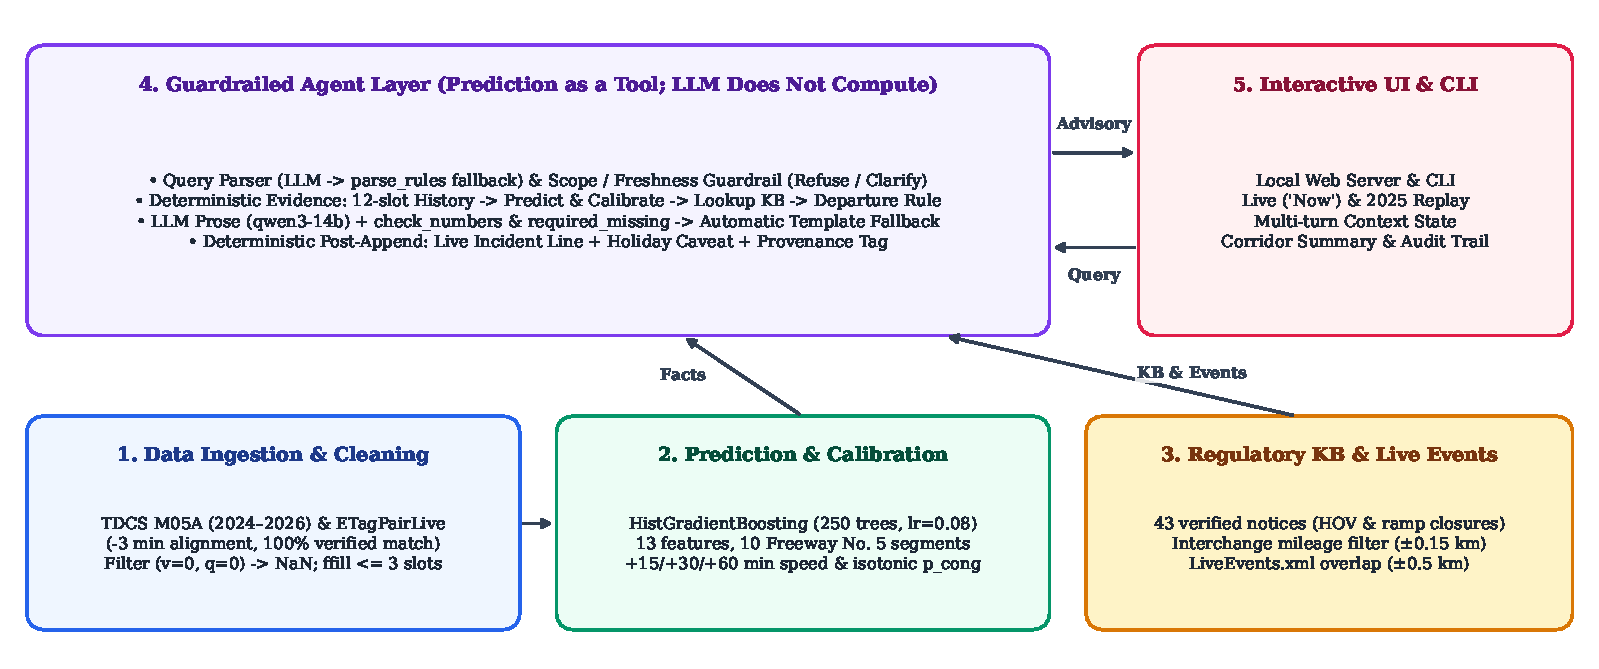
\includegraphics[width=0.95\textwidth]{architecture.pdf}
\caption{Five-module architecture of the explainable tool-augmented Freeway No.~5 congestion prediction agent. Numerical prediction, probability calibration, regulatory matching, and safety verification are executed deterministically outside the LLM.}
\label{fig:architecture}
\end{figure*}

\subsubsection{Module 1: Data Ingestion and Quality-Aware Preprocessing}
Historical archives from TDCS M05A (2024--2026) and live 5-minute XML feeds (\texttt{ETagPairLive.xml}) are normalized into unified daily arrays. Three domain data-quality safeguards are enforced:
\begin{itemize}
    \item \textbf{No-vehicle filtering:} Records with $v_k(t)=0$ and $q_k(t)=0$ (and outlier speeds $>150$~km/h) are converted to \texttt{NaN} rather than 0~km/h, preventing sensor inactivity or zero-flow periods from being mislabeled as extreme congestion.
    \item \textbf{Bounded imputation and cold-start guard:} Missing values are forward-filled up to at most 3 slots (15~min); if any required lag remains missing or $t < 60$ (before 05:00, where 1-hour history and training support are absent), the system refuses to forecast rather than extrapolating.
    \item \textbf{Exact live-to-historical alignment:} Comparing 3,418 passenger-car records on 2026-11-08 established 100\% speed and volume identity under the slot rule $\text{slot} = \lfloor (\text{update\_time} - 3\text{ min}) / 5\text{ min} \rfloor$, whereas unshifted or $-5$/$-8$/$-10$~min alignments yielded only 5\%--88\% agreement. In live mode, feeds older than 20~minutes trigger automatic refusal, and slots timestamped after current time \texttt{now} are excluded.
\end{itemize}

\subsubsection{Module 2: Prediction and Calibration Engine}
For each horizon $h \in \{15, 30, 60\}$~min, we train a scikit-learn \texttt{HistGradientBoostingRegressor} and \texttt{HistGradientBoostingClassifier} (250 boosting iterations, learning rate $0.08$), shared across all 10 segments with segment ID encoded as a categorical feature. Each sample uses 13 features: current speed $v_k(t)$, lagged speeds at $t-\{1,2,3,6,12\}$, 6-slot rolling mean and standard deviation, current volume $q_k(t)$, time-of-day slot, calendar day type (weekday, regular weekend, or long holiday $\ge 3$ consecutive days), holiday day-index (first/middle/final day), and segment ID. Day types are derived strictly from official 2024--2026 calendars so missing cache days never distort holiday classification.

Because raw classifier scores exhibited severe overconfidence during free-flow periods (predicting $\ge 0.9$ on 182 instances with 0 actual congestions), we fit group-wise isotonic regression calibrators~\cite{zadrozny2002isotonic} on held-out 2025 H1 data, stratified by $s_{k,t}$ (currently free-flow vs.\ otherwise) and horizon $h$.

\subsubsection{Module 3: Verified Regulatory Knowledge Base and Live Incidents}
We maintain a structured JSON knowledge base (\texttt{announcements.json}) containing 43 verified traffic-control announcements across 2024 (3), 2025 (20), and 2026 (20), covering HOV restrictions (e.g., 13:00--18:00 northbound at Suao, Luodong, Yilan, and Toucheng ramps) and southbound ramp closures (Shiding and Pinglin). Each record stores applicable dates, road, direction, active time window, verbatim text, source URL, and provenance level (\textit{official notice} vs.\ \textit{media relay}). Announcements are matched to queried segments via interchange mileage with $\pm 0.15$~km tolerance, distinguishing \textit{active} vs.\ \textit{starting within 60~min} rules. In live mode, \texttt{LiveEvents.xml} is parsed to attach direction-matched Freeway No.~5 incidents overlapping the segment ($\pm 0.5$~km). Because neither regulations nor incidents enter the ML feature matrix, they are explicitly presented alongside predictions with clear disclosure.

\subsubsection{Module 4: Guardrailed Agent Layer}
The agent follows a deterministic pipeline (\texttt{Understand} $\rightarrow$ \texttt{Plan} $\rightarrow$ \texttt{Acquire} $\rightarrow$ \texttt{Analyze} $\rightarrow$ \texttt{Lookup} $\rightarrow$ \texttt{Compose}), detailed in Algorithm~\ref{alg:agent}. An OpenAI-compatible local LLM (\texttt{qwen/qwen3-14b} via LM Studio) is used only in two bounded places: (1) extracting structured slots (road, origin, destination, time) from user queries, with automatic fallback to deterministic regular-expression parsing (\texttt{parse\_rules}) while date, direction, and out-of-scope intent are always resolved in code; and (2) composing concise natural-language advice from a serialized \texttt{facts\_text} bundle.

To eliminate numerical hallucination, every LLM response must pass two deterministic validators:
\begin{itemize}
    \item \texttt{check\_numbers}: Every numeric token in the generated text must appear in \texttt{facts\_text} (with standard horizon constants 15, 30, 60 permitted).
    \item \texttt{required\_missing}: The response must retain the rule-selected waiting interval and any active announcement time window.
\end{itemize}
If either check fails or the LLM endpoint is unreachable, the agent transparently falls back to a deterministic template. Finally, live incident lines and holiday accuracy caveats are appended programmatically \textit{after} LLM generation (prompted by empirical testing showing that the LLM omitted holiday caveats in 60\% of holiday queries when left unguarded).

\subsubsection{Module 5: Interactive Presentation}
Both a local Web UI (\texttt{server.py}) and CLI (\texttt{ask.py}) support live (``now'') queries, 2025 historical replay, multi-turn context carryover (date, time, direction, origin), and corridor-wide summary tables, always tagging each response with its provenance (\texttt{[LLM]} or \texttt{[Template: reason]}).

\subsection{Core Advisory Algorithm}
Algorithm~\ref{alg:agent} formalizes the end-to-end decision and verification logic. Candidate departure times $\Delta \in \{0, 15, 30, 60\}$~min are ranked deterministically by minimizing calibrated congestion probability rounded to $0.1$ (ties broken by earliest departure): if $\max_h \hat{p}_k(t+h) < 0.3$, the agent advises departing now; if the minimum candidate risk is $\ge 0.6$, it warns that no smooth window exists within 60~min; otherwise it recommends departing at $\Delta^*$.

\begin{algorithm}[t]
\caption{Guardrailed Congestion Prediction and Advisory Pipeline}
\label{alg:agent}
\begin{algorithmic}[1]
\Require User query $Q$, conversation state $S$, mode $m \in \{\text{live}, \text{replay}\}$
\Ensure Verified advisory response $R$ with provenance tag
\State $P \gets \text{ParseQuery}(Q, S)$ \Comment{LLM extractor; fallback \texttt{parse\_rules}}
\State Resolve date, direction, and intent deterministically from $Q, S$
\If{road $\neq$ Freeway~5 \textbf{or} unsupported intent/year}
    \State \Return $\text{RefuseWithScope}(P)$
\ElsIf{missing required date, time, or direction}
    \State \Return $\text{ClarifyMissing}(P)$
\EndIf
\If{$m = \text{live}$ \textbf{and} ($\text{age} > 20\text{ min}$ \textbf{or} $\text{time} < \text{05:00}$)}
    \State \Return $\text{RefuseDataUnavailable}()$
\EndIf
\State $\mathbf{H} \gets \text{GetRecent}(k, t, 12)$ \Comment{Quality-cleaned 60-min history}
\State $\mathbf{X} \gets \text{BuildFeatures}(\mathbf{H}, \text{calendar\_day\_type}(T))$
\If{$\mathbf{X}$ invalid (insufficient data)}
    \State \Return $\text{ReportInsufficientData}()$
\EndIf
\State $\{\hat{v}_k(t+h), \hat{p}_k(t+h)\}_{h \in \{15,30,60\}} \gets \text{PredictAndCalibrate}(\mathbf{X})$
\State $\mathcal{A} \gets \text{LookupKB}(\text{road}, \text{dir}, T, \text{seg\_km} \pm 0.15)$
\State $d^* \gets \text{SelectDepartureRule}(\{\hat{p}_k(t+h)\})$
\State $F \gets \text{SerializeFacts}(\hat{v}, \hat{p}, \mathcal{A}, d^*, \text{limitations})$
\State $R_{\text{raw}} \gets \text{ComposeLLM}(F)$
\If{\textbf{not} $\text{CheckNumbers}(R_{\text{raw}}, F)$ \textbf{or} $\text{RequiredMissing}(R_{\text{raw}}, d^*, \mathcal{A})$}
    \State $R_{\text{core}} \gets \text{ComposeTemplate}(F)$ \Comment{Deterministic fallback}
\Else
    \State $R_{\text{core}} \gets R_{\text{raw}}$
\EndIf
\State $R \gets \text{AppendFixed}(R_{\text{core}}, \text{Events}, \text{HolidayNote}, \text{Tag})$
\State \Return $R$
\end{algorithmic}
\end{algorithm}
